\section{Results}
\label{sec:results}

The model generated by the Koopman system identification method has a total RMSE averaged across position states and velocity states of {5.98~mm} and {3.66~mm/s}, respectively.
As shown in Table \ref{tab:RMSE}, this corresponds to a total NRMSE averaged across all states of 2.1\%. 
By this metric, it performs more than twice as well as the best competing linear and nonlinear models which have average NRMSEs of 4.6\% and 4.5\%, respectively (see Fig.~\ref{fig:comparison}).
% Fig. \ref{fig:comparison} shows the NRMSE of each model over all states and all trials as compared to the validation data.
The Koopman model also exhibits the smallest standard deviation of the NRMSE across states.
This implies that the Koopman model more consistently captures the real behavior of all six states of the system, rather than just a subset of them.
Fig. \ref{fig:koopmanSim} illustrates the ability of the Koopman-based model to predict the position of the end effector over a 30 second time horizon.

% \David{I feel your results should start with what is obvious to you: IT WORKS. It converges.  You get a result. The result can predict behavior with an accuracy of XYZ.  It took x long to get this result.  If you used different seeds, you always get the same answer (because linear fitting).  Don't forget that you are doing this for the first time and it is important to note that it works.  People will ask themselves how well it works and how they can use it.  Do you need to tune stuff?  Do you need to carefully select parameters or initial guesses?}
% \David{Can you quantify the level of `non-linearity' of your robot?  This would be very valuable for a reader who wants to understand if this nonlinear approach is even necessary.  Can you discuss which of the other methods are linear/ nonlinear.}


%% FIGURE: Koopman simulation plot
\begin{figure}
    \centering
    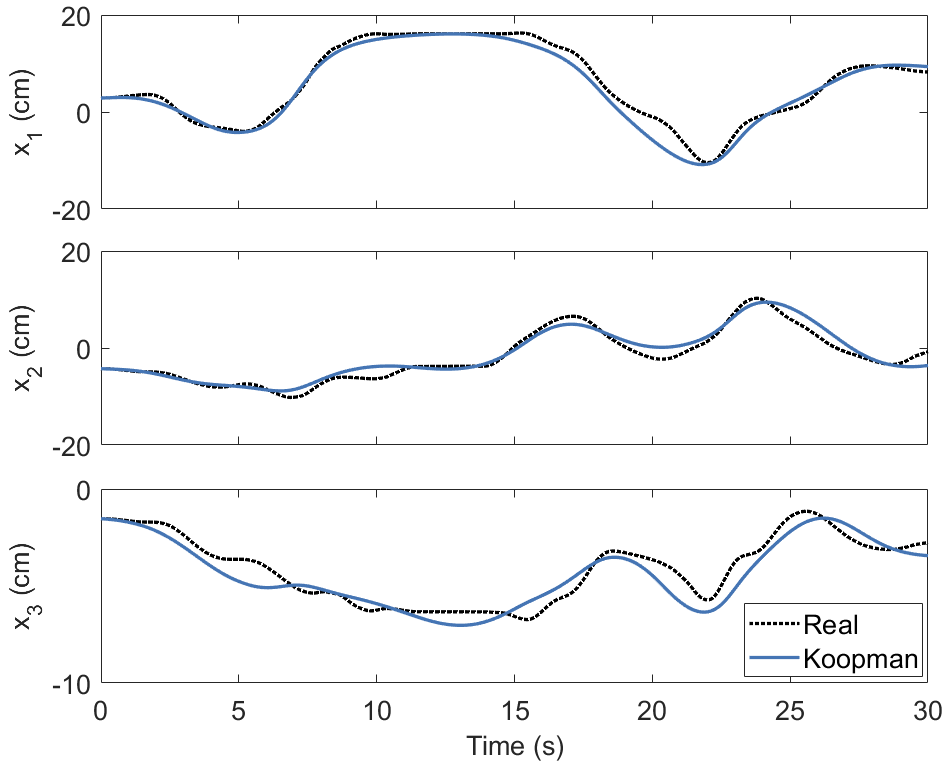
\includegraphics[width=\linewidth]{figures/koopPlot4_cropped.png}
    \caption{
    The measured position of the robot end effector over a 30 second time window (black,dotted) superimposed with the position predicted by the Koopman-based model (blue) given the same initial condition and control inputs.}
    \label{fig:koopmanSim}
\end{figure}

%% FIGURE: Comparison bar graph
\begin{figure}
    \centering
    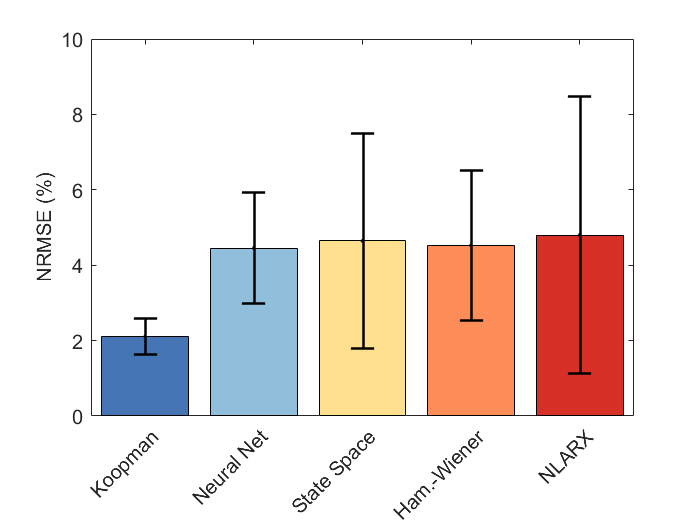
\includegraphics[width=\linewidth]{figures/NRMSE2.png}
    \caption{Shown is the total NRMSE averaged across all states for each of the models, with the standard deviation designated by the black bar. The average NRMSE of the Koopman-based model is less than half of that of the other models, with a standard deviation of less than one third of the other models.}
    \label{fig:comparison}
\end{figure}

%% TABLE: RMSE results table
\begin{table}[]
    \rowcolors{2}{white}{gray!25}
    \setlength\tabcolsep{5pt} % default value: 6pt
    \centering
    \caption{Total NRMSE (\%) over all validation trials}
    \begin{tabular}{|c|c|c|c|c|c|c|c|c|}
        \hline
        \rowcolor{white} 
        & \multicolumn{6}{c |}{\textbf{States}} & & \textbf{Std.} \\
        \cline{2-7} \rowcolor{white}
        \multirow{-2}{*}{\textbf{Model}} & $x_1$ & $x_2$ & $x_3$ & $x_4$ & $x_5$ & $x_6$ & \multirow{-2}{*}{\textbf{Avg.}} & \textbf{Dev.} \\
        \hline
        % RESULTS FOR ROBOT A
        Koopman     &  2.4  &  2.0  &  2.9  &  1.7  &  1.5  &  2.0 & 2.1 & 0.5 \\
        Neural Net  &  5.8  &  4.0  &  6.6  &  3.9  &  2.8  &  3.5 & 4.5 & 1.5 \\
        State Space &  5.1  &  3.1  &  9.9  &  3.0  &  1.8  &  4.8 & 4.6 & 2.9 \\
        Ham.-Weiner &  7.0  &  4.5  &  6.9  &  3.0  &  2.3  &  3.1 & 4.5 & 2.0 \\
        % \multirow{-5}{*}{\cellcolor{white} \rotatebox[origin=c]{90}{\textbf{Robot A}}}
        NLARX       &  5.0  &  3.0 &  12.0  &  3.8  &  2.1  &  2.8 & 4.8 & 3.7 \\
        \hline
        % % RESULTS FOR ROBOT B
        % \cellcolor{white} & Koopman & & & & & & & & \\
        % \cellcolor{white} & Neural Net & & & & & & & & \\
        % \cellcolor{white} & State Space & & & & & & & & \\
        % \cellcolor{white} & Ham.-Weiner & & & & & & & & \\
        % \multirow{-5}{*}{\cellcolor{white} \rotatebox[origin=c]{90}{\textbf{Robot B}}}
        % & NLARX & & & & & & & & \\
        % \hline
    \end{tabular}
    \label{tab:RMSE}
\end{table}